\documentclass[uplatex,dvipdfmx,a4paper,10pt]{jsarticle}

\usepackage{amsmath,amsthm,amssymb}
\usepackage[dvipdfmx]{graphicx}
\usepackage{bm}
%
\usepackage{multirow}
\usepackage{wrapfig}

\usepackage{geometry}
\geometry{left=25truemm, right=25truemm, top=25truemm, bottom=25truemm}

%
\abovecaptionskip=-1pt
%\belowcaptionskip=-1pt
%
\renewcommand{\baselinestretch}{0.84} %全体の行間調整
\renewcommand{\figurename}{Fig.}
\renewcommand{\tablename}{Tab.}
%
\makeatletter 
\def\section{\@startsection {section}{1}{\z@}{1.5 ex plus 2ex minus -.2ex}{0.5 ex plus .2ex}{\large\bf}}
\def\subsection{\@startsection{subsection}{2}{\z@}{0.2\Cvs \@plus.5\Cdp \@minus.2\Cdp}{0.1\Cvs \@plus.3\Cdp}{\reset@font\normalsize\bfseries}}
\makeatother 
%

\renewcommand{\thefootnote}{\fnsymbol{footnote}}

\pagestyle{empty}

\graphicspath{{../../figures//}}

\begin{document}

%%%%%%
% はじめに
%%%%%%
\begin{center}
{\Large \textgt{ランダムな接続性を有するネットワークポリマーの緩和挙動}}
\end{center}

\begin{flushright}
東亞合成 ${}^\circ$佐々木裕
\end{flushright}

% \renewcommand{\thefootnote}{\fnsymbol{footnote}}
\footnote[0]{
{\bf Relaxation Characteristics of Network Polymers with random connectivity using Molecular Dynamics Simulations} \\
\underline{Hiroshi SASAKI} (Toagosei Co., Ltd. 8, Showa-Cho, Minato-ku, NAGOYA 455-0026, JAPAN)\\
Tel: +81-52-611-9923, e-mail: hiroshi\_sasaki$@$mail.toagosei.co.jp
}

\vspace{-3mm}
\section{はじめに}
\subsection{しなやかなネットワークポリマー}

省エネルギーの観点から自動車を中心とした輸送機器の大幅な軽量化の検討が進められており、その中でCFR(T)Pをはじめとする様々な新素材を用いたマルチマテリアル化の鍵の一つとして接着接合技術が注目されている。
接着剤の主成分には、1分子中に複数の反応性官能基を有する反応性オリゴマーが用いられており、光や熱などの外部刺激により速やかにネットワーク構造を形成し、優れた機械的特性を示す。
この場合、接着剤として使用されるネットワークポリマーに要求される特性は、一次的な機械的物性が高いだけでなく、長期間の使用における耐久性を確保するために、様々な変形速度で繰り返し変形させる疲労試験に耐えることが要求される。このような考え方から、脆性破壊を起こしやすい硬い機械物性ではなく、しなやかな強度と延性を兼ね備えたネットワークポリマーが注目されている。

From the viewpoint of energy conservation, significant weight reduction of transportation equipment, especially automobiles, is being considered. In this context, adhesive bonding technology is attracting attention as one of the keys to multi-materialization using CFR(T)P and various other new materials.
Reactive oligomers with multiple reactive functional groups in one molecule are used as the main components of adhesives, which quickly form a network structure upon external stimuli such as light or heat, and exhibit excellent mechanical properties.
In this case, the properties required of network polymers used as adhesives are not only high primary mechanical properties, but also the ability to withstand fatigue tests in which the polymer is repeatedly deformed at various deformation rates in order to ensure durability in long-term use. Based on this concept, network polymers that combine supple strength and ductility, rather than hard mechanical properties that are prone to brittle fracture, are attracting attention.


\subsection{力学的ヒステリシスの重要性}

材料の耐久性を確保するためには機械的性質の発現機構とその劣化メカニズムを解明する必要があり、金属などのハードな材料では破壊工学として体系化されている。
破壊工学の概念を端的に表現すると、「系内に欠陥が存在することを前提とした耐久性の評価」である。破壊挙動は、材料の脆性破壊を仮定した「グリフィス理論」における亀裂進展に伴うエネルギー放出速度である$G_c$と、$J$積分により非線形領域に拡張された$J_c$で議論され、これらの値が靭性の指標とされている。
しかし、破壊時の変形が極めて大きいソフトマター材料への適用には注意が必要である。

旧知のソフトな材料であるゴムの破壊靭性が大きい原因として、その破壊エネルギーが応力-ひずみ関係における機械的ヒステリシスロスと良い相関を示すことが報告されている~\cite{payne1}。
Andrewsは、応力-ひずみ関係における機械的ヒステリシスに着目し、ヒステリシス損失によりき裂進展に伴うエネルギー放出が減少し、結果としてき裂進展が抑制されるというモデルを提案した~\cite{Andrews}。
Payneは、ヒステリシスロスの発現機構を、1) 粘弾性に基づくもの、2) 結晶化に基づくもの、3) フィラー添加によるもの、の3つの主要なメカニズムに分類した~\cite{payne2}。
ヒステリシスの原因として、フィラー由来、あるいは、伸張結晶化のようなメゾスケール領域の挙動に注目する場合が多く見受けられる~\cite{zhang, Igarashi2013}。
また、超高強度ゲルとして知られているダブルネットワークゲル中の犠牲結合においても、大きなヒステリシスが見られる~\cite{Gong2010}。

上述したこれまでの検討は分子鎖の描写よりもわずかに大きいメソスケール領域に注目しており、この比較的大きなスケールでの挙動は、一般に長い緩和時間をもたらす。
ヒステリシス挙動はこのスケールでのみ起こるのだろうか?
われわれは、機械的ヒステリシスはより微視的な分子鎖の描像でも起こり、その結果、速い周期の刺激に対する破壊抵抗性と関連していると考えている。

一般に、破壊試験による材料の強度評価は任意の変形速度での一回の変形挙動で評価されるため、ヒステリシスの回復挙動の遅速はあまり問題にならない。
しかしながら、材料としての耐久性を保証するためには、多様な変形速度での繰り返し変形を行う疲労試験に対する耐久性も重要である。
この場合、適正な緩和時間で回復する可逆的なメカニズムに基づく強靭化機構が必要となる。


To ensure the durability of materials, it is necessary to elucidate the mechanism of mechanical property development and its degradation mechanism, which is systematized as fracture engineering for hard materials such as metals.
The concept of fracture engineering can be simply expressed as "evaluation of durability based on the assumption that defects exist in the system". Fracture behavior is discussed in terms of $G_c$, which is the energy release rate associated with crack propagation in "Griffith Theory," which assumes brittle fracture of materials, and $J_c$, which is extended to the nonlinear region by $J$ integration, and these values are used as indicators of toughness.

However, caution must be exercised in applying this method to soft-matter materials, which are subject to extremely large deformation at fracture.
As a cause of the large fracture toughness of rubber, an old soft material, it has been reported that its fracture energy shows a good correlation with the mechanical hysteresis loss in the stress-strain relationship~\cite{payne1}.
Andrews focused on mechanical hysteresis in the stress-strain relationship and proposed a model in which hysteresis loss reduces the energy release associated with crack growth and consequently suppresses crack growth.
Payne classified hysteresis loss into three main mechanisms: 1) viscoelasticity-based, 2) crystallization-based, and 3) filler addition.
Hysteresis is often attributed to filler origin or to meso-scale region behavior such as elongational crystallization~\cite{zhang, Igarashi2013}.
Large hysteresis is also observed in sacrificial bonding in double network gels, known as ultra-high-strength gels~\cite{Gong2010}.

Previous investigations described above have focused on mesoscale regions that are slightly larger than the molecular chain depiction, and behavior at this relatively large scale generally leads to long relaxation times.
Does hysteresis behavior occur only at this scale?
We believe that mechanical hysteresis also occurs in more microscopic molecular chain depictions and is thus associated with fracture resistance to fast-periodic stimuli.

In general, the slow recovery behavior of hysteresis is not a major issue since the strength evaluation of a material by fracture testing is based on a single deformation behavior at an arbitrary deformation rate.
However, in order to assure the durability of a material, it is also important to have durability against fatigue tests in which the material is repeatedly deformed at various deformation rates.
In this case, a toughening mechanism based on a reversible mechanism that recovers with an appropriate relaxation time is required.

Translated with www.DeepL.com/Translator (free version)

\subsection{破壊にたいする粘弾性効果}
ゴム系材料の破壊において時間温度換算則が大変形を伴う破壊挙動にも成立し、室温では容易に破断する SBR がガラス転移温度に近い低温での伸長では高い伸びと強度を示すことも報告されている~\cite{smith}。
この時間温度換算則については粘弾性効果に基づくものとして取り扱うべきであり、その由来をミクロな分子描像で記述できるかもしれない。

It has been reported that Time-Temperature Superposition Rule holds true for the fracture behavior of rubber-based materials with large deformation, and that SBR, which breaks easily at room temperature, shows high elongation and strength when elongated at low temperatures close to its glass transition temperature~\cite{smith}.
This Time-Temperature Superposition Rule should be treated as based on viscoelastic effects, and its origin may be described by microscopic molecular description.


\subsection{各種のネットワークモデル}


ゴム弾性の古典的なモデルである ``Affine Network Model'' からの発展形として、結節点の揺らぎに注目した``Phantom Network Model: PNM''が提案され、Flory によればメルト状態と同一なストランドのゆらぎを有するランダムネットワークにおいて PNM のふるまいを示すとされている~\cite{flory}。
我々は、この結節点のゆらぎ由来の散逸が、分子鎖描像のようなミクロなスケールでの粘弾性的なエネルギー散逸モデルとなりうるのではないかと考え、これまで検討を進めている~\cite{sasaki}。




\subsection{目指すもの}




\subsection{本検討内容}
(本検討内容)
ソフトマターの構造材料への展開を標語的に言えば、「脆性破壊を伴いがちな剛直性から、設計された延性に基づく高耐久性を示す『しなやかな強さ』へのパラダイムシフト」となるであろう。
この設計された延性に必要な要件を明確にすることが本研究の目的である。

本報告では、先行研究である Everaers らの方法~\cite{Everaers1999} に従った規則構造を有するネットワークの分子動力学(MD)シミュレーションによりそのゴム弾性挙動の変形速度依存性と緩和時間との関連について検討を行い、時間温度換算則が成り立つような線形粘弾性の枠組みでのヒステリシスを考察した。







ネットワークポリマー研究の深化と新規材料への展開


\subsection{ネットワークポリマーの破壊}



\subsection{``Phantom Network Model'' の確認}
``Phantom Network Model: PNM''





以前に、規則構造ネットワークをベースとしてユニットセル間における規則性をランダムへと変えることで架橋欠損のないネットワークを作成して PNM を再現できることを報告した~\cite{sasaki}。



本報告では、ランダムな接続性を有するネットワークポリマーの緩和挙動について、MD シミュレーションにより検討した結果について報告する。






近年、ソフトマターの階層的な構造設計の考え方が深化し、力学特性に優れたネットワークポリマーの材料設計にも応用されている。
旧知の材料であるゴムの大きな破壊靭性の由来については、 ヒステリシスロスのようなエネルギー散逸により亀裂進展が抑制されるという Andrews モデルが提案されている\cite{andrews}。
また、ゴム系材料の破壊において粘弾性挙動として時間温度換算則が大変形を伴う破壊挙動にも成立し、室温では容易に破断する SBR がガラス転移温度に近い低温での伸長では高い伸びと強度を示すことも報告されている~\cite{smith}。

ゴム弾性の古典的なモデルである ``Affine Network Model'' からの発展形として、結節点の揺らぎに注目した``Phantom Network Model: PNM''が提案され、Flory によればメルト状態と同一なストランドのゆらぎを有するランダムネットワークにおいて PNM のふるまいを示すとされている~\cite{flory}。
我々は、この結節点のゆらぎ由来の散逸が、分子鎖描像のようなミクロなスケールでの粘弾性的なエネルギー散逸モデルとなりうるのではないかと考え、これまで検討を進めている。



以前に、規則構造ネットワークをベースとしてユニットセル間における規則性をランダムへと変えることで架橋欠損のないネットワークを作成して PNM を再現できることを報告した~\cite{sasaki}。
本報告では、ランダムな接続性を有するネットワークポリマーの緩和挙動について、MD シミュレーションにより検討した結果について報告する。






\vspace{-1mm}
\section{結果}
\subsection{シミュレーションについて}
既報~\cite{sasaki}に従い、ランダムな接続性を有する 4 および 3 分岐のネットワークを作成し、その平衡状態および変形(一軸伸張およびずりせん断)時の振る舞いについて、OCTA 上の COGNAC シミュレーターを用いた分子動力学シミュレーションにより評価した。


% \subsection{ネットワークの線形粘弾性}
% 変形速度を変化させた場合の SS カーブを Fig.\ref{fig:stretch} に示した。
% 平衡状態の MD シミュレーションから Green-Kubo 公式により求めたネットワークの応力緩和関数(赤線)および $\nu k_B T$ から算出したゴム弾性プラトーの値を緩和関数から差し引いたもの(緑線)を併せて Fig.\ref{fig: Relux} に示した。
% また、ストランドと同等な自由鎖(N=46)のラウス緩和(最長ラウス緩和時間 $\tau_R = 2700$)についても示している。

% この類似性から、少なくとも、今回検討した単純な規則構造を有するネットワークにおいては、架橋構造の緩和時間への寄与は少ないものと推定できた。

% % \begin{wrapfigure}{r}{65mm}
% % %\vspace{-1\baselineskip}
% % 	\begin{center}
% % 	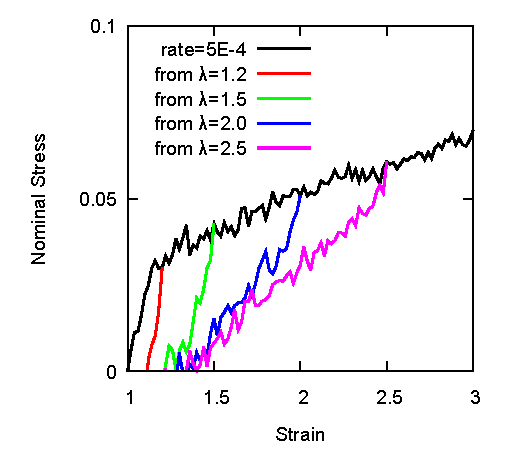
\includegraphics[width=60mm]{./fig/N44_rev_SS.pdf}
% % 	\caption{Hysteresis Curves from different elongation position}
% % 	\label{fig: hyst}
% % 	\end{center}
% % \vspace{-5mm}
% % \end{wrapfigure}

\subsection{力学応答の評価}
4 分岐のネットワークポリマーに対して、変形速度の異なるせん断変形(1e-2 $\sim$ 5e-5 $\lambda/\tau$)時の SS カーブを、各種モデルの理論曲線と共に Fig. \ref{fig:deform} に示した。
変形速度の低減により、$\lambda<1$ 程度の小さなひずみでは PNM に漸近していた。
PNM へと漸近する変形速度 (2e-4 $\lambda/\tau$) で周期的なせん断変形 ($\lambda = 1$) を付与した結果(Fig. \ref{fig:hyst})においても、複数回の変形に対しても迅速な回復を伴った力学的ヒステリシス (Hysteresis loss $\simeq$ 35\%) を示すことが確認できた。
% また、伸長速度を遅くすることにより、ヒステリシス強度が減少することも確認できた。

変形モードの違いによって上記の挙動が変化することも見出しており、その詳細についても報告予定である。

% \section{おわりに}

% 本報告においては、単純な規則構造を有するネットワークの線形緩和現象と任意の変形速度での力学応答との関係から力学的ヒステリシスが生じることを確認し、その発現メカニズムがストランドの緩和現象に起因するものであることを推定した。
% 実際の破壊現象はこれほど単純ではなく、大変形時の非線形応答を考慮する必要は大きいと考えている。
% さらなる検討を進めていきたい。


\begin{figure}[hb]
    \begin{minipage}{0.5\hsize}
        \begin{center}
        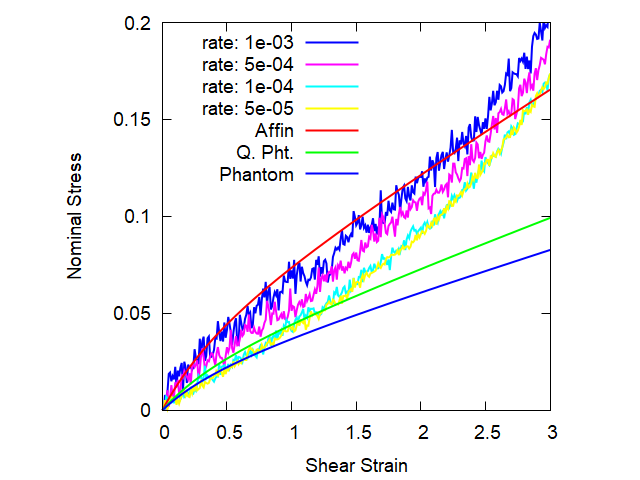
\includegraphics[width=.7\textwidth]{Shear_Random_4chain_N20.png}
        \caption{Stress-Strain Curves for 4-chain NW at varied shear rate (1e-2 $\sim$ 5e-5 $\lambda/\tau$)}
        \label{fig:deform}
        \end{center}
    \end{minipage}
    \begin{minipage}{0.5\hsize}
        \begin{center}
        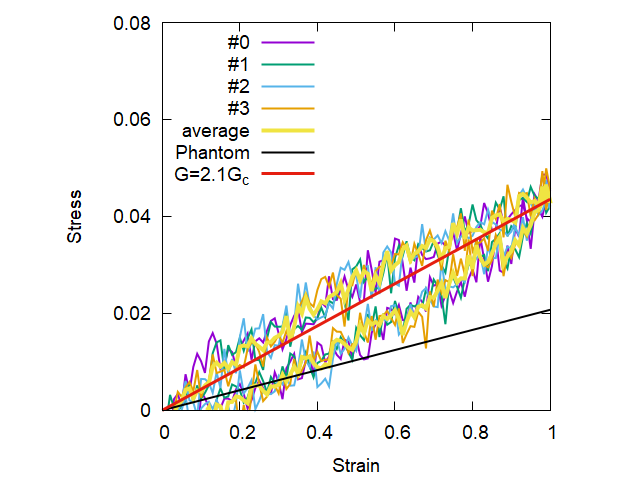
\includegraphics[width=.7\textwidth]{CyclicDeform_4chain_rate_2e-4.png}
        \caption{Hysteresis Curves for 4-chain NW by Cyclic Shear ($\lambda = 1$): shear rate 2e-4 $\lambda/\tau$}
        \label{fig:hyst}
        \end{center}
    \end{minipage}
    % \begin{minipage}{0.33\hsize}
    %     \begin{center}
    %     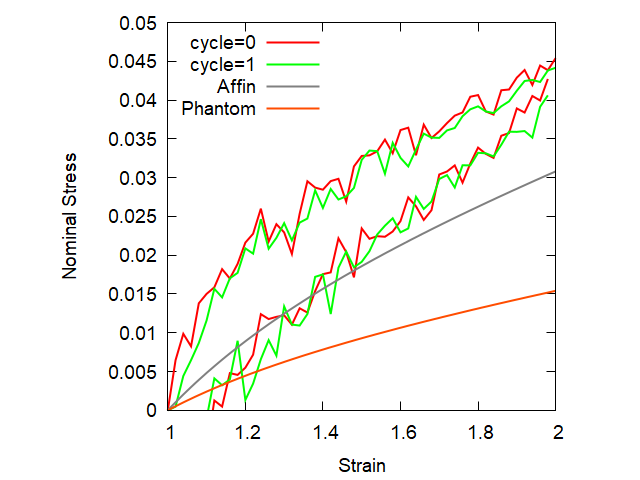
\includegraphics[width=\textwidth]{hyst_4Chain.png}
    %     \caption{Strand Exchange Procedure}
    %     \label{fig:exc}
    %     \end{center}
    % \end{minipage}
\end{figure}

\vspace{-7mm}
\begin{thebibliography}{99}
    \bibitem{payne1} K. Grosch, J.A.C. Harwood \& A.R. Payne, Nature, 212 5061 497 (1966)
    \bibitem{andrews} E. H. Andrews, Y. Fukahori, J. of Mat. Sci., 12, 1307 (1977)
    \bibitem{payne2} A. R.Payne, J. Polym. Sci. Part C, Polym. Symp., 48(48), 169 (1974)
    \bibitem{zhang} H. Zhang et al. Macromolecules 46, 900 (2013)
    \bibitem{smith} T. L. Smith, R. A. Dickie, J. of Polym. Sci. A-2: Polym. Phys., 7, 635 (1969)
    \bibitem{flory} P. J. Flory, Proc. R. Soc. London. Series A, 351, 351 (1976)
    \bibitem{sasaki} 佐々木裕, 第69回レオロジー討論会 (2021)
    \bibitem{Auhl} R. Auhl et al., J. of Chem. Phys., 119, 12718 (2003)
    \bibitem{Kroger} S. Shanbhag, M. Kr\"{o}ger, Macromol. 40 2897 (2007)
    \bibitem{rubinstein} J. T. Kalathi et al., Macromol. 47 6925 (2014)
    \bibitem{flory} P. J. Flory Proceedings of the Royal Society of London. Series A, 351, 351 (1976)
    \bibitem{sasaki} 佐々木裕, 第69回レオロジー討論会 要旨集 (2021)
\end{thebibliography}

\end{document}